% Created by Takeuchi on May. 2021
\documentclass[dvipdfmx, 11pt]{beamer}

%%%% Packages %%%%%
%\usepackage{bxdpx-beamer}
%\usepackage{minijs}
%\usepackage{otf}
%\usepackage{tabularx}
%\usepackage{graphicx}
% \usepackage{graphicx}
% \usepackage{amsmath,amssymb,amsthm}
% \usepackage{multirow}
\usepackage{multicol}
% \usepackage{url}
\usepackage{tikz}
\usetikzlibrary{arrows,shapes}
\usetikzlibrary{positioning}
% \usepackage{alltt}
% \usepackage{bm}
 \usepackage{listings,jlisting}
% \usepackage{listings}
% \lstset{
%  basicstyle=\ttfamily\scriptsize,
%  keepspaces=true,
%  escapechar=|,
%  columns=[l]{fullflexible}
% }

%%%% Fonts %%%%%
\renewcommand{\kanjifamilydefault}{\gtdefault}
 %\usepackage{otf} % otfパッケージ
 \usepackage[deluxe]{otf} 
%\renewcommand{\kanjifamilydefault}{mg}
\usepackage{txfonts} % 数式・英文ローマン体を Lxfont にする
% \usepackage[T1]{fontenc} % 8bit フォント
% \usepackage{minijs}
% \usepackage{textcomp} % 欧文フォントの追加
% \usepackage[utf8]{inputenc} % 文字コードをUTF-8

%%%%% Beamer %%%%%
\usetheme{Madrid}
\useinnertheme{rectangles}
%\useoutertheme{smoothbars}
\setbeamercolor{enumerate}{fg=white, bg=black}
\usefonttheme{professionalfonts}
\setbeamertemplate{frametitle}[default][center]
\setbeamertemplate{navigation symbols}{}
% \setbeamercovered{transparent} % 好みに応じてどうぞ
\setbeamertemplate{footline}[frame number]
\setbeamercolor{page number in head/foot}{fg=black} % ページ数を表示する
% \setbeamerfont{footline}{size=\normalsize,series=\bfseries}
\setbeamerfont{footline}{size=\scriptsize,series=\mdseries}
\setbeamercolor{footline}{fg=black,bg=black}
\setbeamertemplate{blocks}[rounded][shadow=true]
\setbeamertemplate{items}[ball]
% \setbeamertemplate{enumerate items}[default]
% \setbeamerfont{alerted text}{series=\bfseries}
\newcommand{\backupbegin}{
   \newcounter{framenumberappendix}
   \setcounter{framenumberappendix}{\value{framenumber}}
}
\newcommand{\backupend}{
   \addtocounter{framenumberappendix}{-\value{framenumber}}
   \addtocounter{framenumber}{\value{framenumberappendix}} 
}
\renewcommand{\thefootnote}{\dag} % フットノート番号をダガーにする

%%%% Code %%%%%%%%%
\lstset{
 basicstyle=\ttfamily\color{black},
 keepspaces=true,
 escapechar=|,
 columns=[l]{fullflexible},
 commentstyle={\color{red}},
 stringstyle={\color{blue}},
 % literrate =%
 %   {:-}{{\textcolor{black}{:-}}}2%
 %   {,}{{\textcolor{black}{,}}}1%
 %   {.}{{\textcolor{black}{.}}}1%
}

%%%% My macro %%%%%
%%%%%%%%%%%%%%%%%%%%%%%%%%%%%%%%%%%%%%%%%%%%%%%%%%%%%%%%%%%%%%%%
% User-defined Macro
%%%%%%%%%%%%%%%%%%%%%%%%%%%%%%%%%%%%%%%%%%%%%%%%%%%%%%%%%%%%%%%%
\newcommand{\compress}{\itemsep0pt\parsep0pt\parskip0pt\partopsep0pt}
% \newcommand{\compress}{\itemsep1pt plus1pt\parsep0pt\parskip0pt}
% \newcommand{\code}[1]{\lstinline[basicstyle=\ttfamily]{#1}}
\newcommand{\gringo}{\textit{gringo}}
\newcommand{\clasp}{\textit{clasp}}
\newcommand{\clingo}{\textit{clingo}}
\newcommand{\teaspoon}{\textit{teaspoon}}
\newcommand{\sat}{\textsf{SAT}}
\newcommand{\unsat}{\textsf{UNSAT}}
% \newcommand{\web}[2]{\href{#1}{#2\ \raisebox{-0.15ex}{\beamergotobutton{Web}}}}
% \newcommand{\doi}[2]{\href{#1}{#2\ \raisebox{-0.15ex}{\beamergotobutton{DOI}}}}
% \newcommand{\weblink}[1]{\web{#1}{#1}}
% \newcommand{\imp}{\mathrel{\Rightarrow}}
% \newcommand{\Iff}{\mathrel{\Leftrightarrow}}
% \newcommand{\mybox}[1]{\fbox{\rule[.2cm]{0cm}{0cm}\mbox{${#1}$}}}
% \newcommand{\mycbox}[2]{\tikz[baseline]\node[fill=#1!10,anchor=base,rounded corners=2pt] () {#2};}
% \newcommand{\naf}[1]{\ensuremath{{\sim\!\!{#1}}}}
% \newcommand{\head}[1]{\ensuremath{\mathit{head}(#1)}}
% \newcommand{\body}[1]{\ensuremath{\mathit{body}(#1)}}
% \newcommand{\atom}[1]{\ensuremath{\mathit{atom}(#1)}}
% \newcommand{\poslits}[1]{\ensuremath{{#1}^+}}
% \newcommand{\neglits}[1]{\ensuremath{{#1}^-}}
% \newcommand{\pbody}[1]{\poslits{\body{#1}}}
% \newcommand{\nbody}[1]{\neglits{\body{#1}}}
% \newcommand{\Cn}[1]{\ensuremath{\mathit{Cn}(#1)}}
% \newcommand{\reduct}[2]{\ensuremath{#1^{#2}}}
% \newcommand{\OK}{\mbox{\textcolor{green}{\Pisymbol{pzd}{52}}}}
% \newcommand{\KO}{\mbox{\textcolor{red}{\Pisymbol{pzd}{56}}}}
% \newcommand{\code}[1]{\lstinline[basicstyle=\ttfamily]{#1}}
% \newcommand{\lw}[1]{\smash{\lower2.ex\hbox{#1}}}
\newcommand{\llw}[1]{\smash{\lower3.ex\hbox{#1}}}

\newenvironment{tableC}{%
  \scriptsize
  \renewcommand{\arraystretch}{0.9}
  \tabcolsep = 0.6mm
  % \begin{tabular}[t]{p{6mm}|rlr|rlr|rlr|rlr|rlr}\hline
  %   \multicolumn{1}{l|}{\llw{問題   }} &
  \begin{tabular}[t]{l|rlr|rlr|rlr|rlr|rlr}\hline
    \multicolumn{1}{l|}{\llw{問題}} &
    \multicolumn{3}{c|}{UD1} &
    \multicolumn{3}{c|}{UD2} &
    \multicolumn{3}{c|}{UD3} &
    \multicolumn{3}{c|}{UD4} &
    \multicolumn{3}{c}{UD5} \\
    & 
    \multicolumn{1}{c}{既知の} & & \multicolumn{1}{c|}{ASP} & 
    \multicolumn{1}{c}{既知の} & & \multicolumn{1}{c|}{ASP} & 
    \multicolumn{1}{c}{既知の} & & \multicolumn{1}{c|}{ASP} & 
    \multicolumn{1}{c}{既知の} & & \multicolumn{1}{c|}{ASP} & 
    \multicolumn{1}{c}{既知の} & & \multicolumn{1}{c}{ASP} \\
    & 
    ベスト & &  & 
    ベスト & &  & 
    ベスト & &  & 
    ベスト & &  & 
    ベスト & &  \\
    \hline
  }{%
    \hline
  \end{tabular}
}

\newcommand{\nodeVP}[3]{
  \coordinate[#2] (#1);
  \draw[fill=cyan!30] (#1)--+(-1,0)--+(0,1)--+(1,0)--cycle;
  \draw (#1)node[above]{\tiny{#3}};
  \draw[fill=black] (#1) +(-0.5,0.5)--+(0.5,0.5)--+(0,1)--cycle;
  \node[rectangle,above=0.5cm of #1,white](vp){\tiny{VP}};
  \coordinate[below=0.5cm of #1] (via_#1);
  \draw (via_#1)node[above right]{\tiny{[1..1]}};
  \draw (via_#1) +(170:0.2) arc (170:370:0.2);
  \draw (#1)--(via_#1);

}
\newcommand{\nodeTrans}[3]{
  \coordinate[#2] (#1);
  \draw[fill=cyan!30] (#1)--+(-1,0)--+(0,1)--+(1,0)--cycle;
  \draw (#1)node[above]{\tiny{#3}};
  \draw[fill=black] (#1) +(-0.5,0.5)--+(0.5,0.5)--+(0,1)--cycle;
  \node[rectangle,above=0.5cm of #1,white](vp){\tiny{VP}};
  \coordinate[below=1.7cm of #1] (via_#1);
  \draw (via_#1)node[below=0.2cm]{\tiny{[1..1]}};
  \draw (via_#1) +(135:0.2) arc (135:405:0.2);
  \draw (#1)--(via_#1);

}

\newcommand{\nodeVPdashed}[3]{
  \coordinate[#2] (#1);
  \draw[fill=cyan!30,dashed] (#1)--+(-1,0)--+(0,1)--+(1,0)--cycle;
  \draw (#1)node[above]{\tiny{#3}};
  \fill[black] (#1) +(-0.5,0.5)--+(0.5,0.5)-- +(0,1)--cycle;
  \node[rectangle,above=0.5cm of #1,white](vp){\tiny{VP}};
  \coordinate[below=0.5cm of #1] (via_#1);
  \draw (via_#1)node[above right]{\tiny{[1..1]}};
  \draw (via_#1) +(-0.2,0) arc (180:360:0.2);
  \draw (#1)--(via_#1);

}

\newcommand{\nodeV}[4]{
  \node [draw,inner xsep=2pt,#2,fill=black!10,font=\tiny] (#1){
      \begin{tabular}{l}
       #3\\
       #4\\
      \end{tabular}
  };
  \fill [black] (#1.north west)--++(0,-2mm)--++(1mm,0)--++(1mm,0)--++(0,2mm); 
  \draw (#1.north west) ++(1mm,-1mm) node[white]{\tiny{v}};
}

\newcommand{\nodeVchoiced}[4]{
  \node [draw,inner xsep=2pt,#2,fill=red!50,font=\tiny] (#1){
      \begin{tabular}{l}
       #3\\
       #4\\
      \end{tabular}
  };
  \fill [black] (#1.north west)--++(0,-2mm)--++(1mm,0)--++(1mm,0)--++(0,2mm); 
  \draw (#1.north west) ++(1mm,-1mm) node[white]{\tiny{v}};

}

%%%%%%%%%%%%%%%%%%%%%%%%%%%%%%%%%%%%%%%%%%%%%%%%%%%%
\title{解集合プログラミングを用いた\\多目的車両装備仕様問題の解法}
\author{竹内頼人\inst{1} \and 田村直之\inst{2} \and 番原睦則\inst{1}}
\institute{\inst{1}名古屋大学 大学院情報学研究科 \and \inst{2}神戸大学 情報基盤センター}
\date{2021年度 人工知能学会全国大会(第35回)}
\begin{document}
\frame{\titlepage}
%%%%%%%%%%%%%%%%%%%%%%%%%%%%%%%%%%%%%%%%%%%%%%%%%%%%
\begin{frame}{車両装備仕様}
  \begin{alertblock}{車両装備仕様とは}
    簡単に言うと,自動車のカタログに記載されている
    \textbf{車種(モデル/グレード)と装備の組合せ}のことである.
  \end{alertblock}

  \begin{itemize}
  \item 車両装備仕様を決めるには,販売される国や地域の法規や規制,
	地域や市場の特性,市場の嗜好や競合など十分に考慮する必要がある.
  \item 現状では,専門知識をもつ技術者の多大な労力が費やされている.
  \item 車両装備仕様の自動生成は自動車メーカーにとって重要な課題
	の一つである.
  \end{itemize}

  % \begin{block}{車両装備仕様問題 (組合せ最適化問題の一種)}
  %   \begin{itemize}
  %   \item 装備タイプと装備オプションに対する
  %     \structure{\bf 範囲制約},
  %     \structure{\bf 依存制約},
  %     \structure{\bf 燃費制約}
  %     から構成される.
  %   \item 予想販売台数が最大となる装備仕様を求めることが目的である.
  %   \end{itemize}
  % \end{block}
\end{frame}
%%%%%%%%%%%%%%%%%%%%%%%%%%%%%%%%%%%%%%%%%%%%%%%%%%%%
\begin{frame}{CAFE方式 (企業別平均燃費方式)}
 \begin{alertblock}{CAFE方式とは}
  自動車の燃費規制で,車種別ではなくメーカー全体での出荷台数を加味した
  平均燃費を算出し,規制をかける方式.
 \end{alertblock}
 \begin{itemize}
  \item $n$車種の場合,車種$i$の燃費を$FE_i$,予想販売台数を$SV_i$とすると,
    \[
      \begin{array}{lcr}
        \underbrace{
        \frac{\sum_{i=1}^{n} FE_{i}\cdot SV_{i}}
        {\sum_{i=1}^{n} SV_{i}}}_{\textrm{平均燃費}
        }
        &
        \geq 
        &
        \textrm{CAFE基準値($t$)}
      \end{array}
    \]
  \item 特長は,ある車種では燃費基準を達成できなくても,他の車種の燃費を
    向上させることで基準を達成することが可能な点.
  \item 欧米で採用されており,日本でも\structure{\bf 2020年度から導入されている}.
 \end{itemize}
 \footnotetext{本研究では,CAFE方式の計算方法として,単純化された式を扱っている.}
\end{frame}
%%%%%%%%%%%%%%%%%%%%%%%%%%%%%%%%%%%%%%%%%%%%%%%%%%%%
\begin{frame}{多目的車両装備仕様問題}
 \begin{alertblock}{多目的車両装備仕様問題とは}
  \begin{itemize}
   \item 組合せ最適化問題の一種で,装備および燃費に関する制約をもつ.
   % \item 問題インスタンス,燃費テーブル,販売台数テーブル
   \item {\bf 予想販売台数の最大化}や{\bf 装備オプション数の最小化}など,
	 トレードオフの関係にある複数の目的関数のもとで
	 最適な車両装備仕様を求めることが目的
  \end{itemize}
 \end{alertblock}
 \begin{block}{制約}
  \begin{description}
   \item[{\bf 範囲制約}]: 各車種について,各装備タイプで選択される装備オプション数は,
	      与えられた上下限値の範囲内でなければならない.
   \item[{\bf 依存制約}]: 各車種について,装備オプションや装備タイプの間にある依存関係を
	      満たさなければならない.
   \item[{\bf 燃費制約}]: CAFE方式による基準を満たさなければならない.
  \end{description}
 \end{block}
 CAFE方式に基づく多目的車両装備仕様問題(\structure{\bf 多目的CAFE問題})を対象とする.
\end{frame}
%%%%%%%%%%%%%%%%%%%%%%%%%%%%%%%%%%%%%%%%%%%%%%%%%%%%
\begin{frame}{多目的CAFE問題の例}

  \begin{columns}
    \begin{column}{0.75\linewidth}
      \scalebox{0.8}[0.8]{ 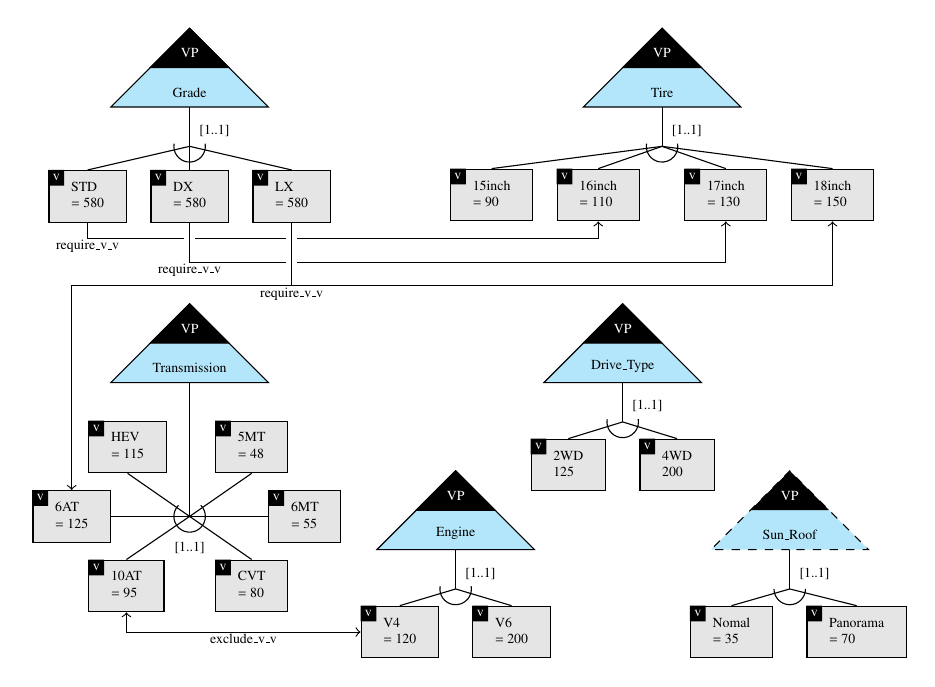
\begin{tikzpicture}
 % Grade
  \nodeVP{grade}{at={(0,0)}}{Grade};
  \nodeV{dx}{below=0.3cm of via_grade}{DX}{= 580};
  \draw(via_grade)--(dx.north);
  \nodeV{std}{left=0.3cm of dx}{STD}{= 580};
  \draw(via_grade)--(std.north);
  \nodeV{lx}{right=0.3cm of dx}{LX}{= 580};
  \draw(via_grade)--(lx.north);

  % Tire
  \nodeVP{tire}{right=6cm of grade}{Tire};
  \nodeV{16inch}{below left=0.4cm of via_tire}{16inch}{= 110};
  \nodeV{17inch}{below right=0.4cm of via_tire}{17inch}{= 130};
  \nodeV{15inch}{left=0.3cm of 16inch}{15inch}{= 90};
  \nodeV{18inch}{right=0.3cm of 17inch}{18inch}{= 150};
  \draw (via_tire)--(15inch.north);
  \draw (via_tire)--(16inch.north);
  \draw (via_tire)--(17inch.north);
  \draw (via_tire)--(18inch.north);

  % Transmission
  \nodeTrans{trans}{below=3.5cm of grade}{Transmission};
  \nodeV{6at}{left=1cm of via_trans}{6AT}{= 125};
  \nodeV{hev}{above right=0.3cm of 6at.north}{HEV}{= 115};
  \nodeV{10at}{below right=0.3cm of 6at.south}{10AT}{= 95};
  \nodeV{6mt}{right=1cm of via_trans}{6MT}{= 55};
  \nodeV{5mt}{above left=0.3cm of 6mt.north}{5MT}{= 48};
  \nodeV{cvt}{below left=0.3cm of 6mt.south}{CVT}{= 80};
  \draw (via_trans)--(10at.north);
  \draw (via_trans)--(6at.east);
  \draw (via_trans)--(hev.south);
  \draw (via_trans)--(6mt.west);
  \draw (via_trans)--(5mt.south);
  \draw (via_trans)--(cvt.north);

  % Drive_Type
  \nodeVP{drivetype}{right=5.5cm of trans}{Drive\_Type};
  \nodeV{2wd}{below left=0.3cm of via_drivetype}{2WD}{125};
  \draw (via_drivetype)--(2wd.north);
  \nodeV{4wd}{below right=0.3cm of via_drivetype}{4WD}{200};
  \draw (via_drivetype)--(4wd.north);


  % Sun_Roof
  \nodeVPdashed{sunroof}{below right=3cm of drivetype}{Sun\_Roof};
  \nodeV{nomal}{below left=0.3cm of via_sunroof}{Nomal}{= 35};
  \draw (via_sunroof)--(nomal.north);
  \nodeV{panorama}{below right=0.3cm of via_sunroof}{Panorama}{= 70};
  \draw (via_sunroof)--(panorama.north);

  % Engine
  \nodeVP{engine}{below left=3cm of drivetype}{Engine};
  \nodeV{v4}{below left=0.3cm of via_engine}{V4}{= 120};
  \draw (via_engine)--(v4.north);
  \nodeV{v6}{below right=0.3cm of via_engine}{V6}{= 200};
  \draw (via_engine)--(v6.north);
  
 

  % require
  \draw[->] (std.south)--++(0,-0.2) node[below=-1mm] {\tiny{require\_v\_v}} -|(16inch.south);
  \draw[white,line width=4pt](dx.south) ++(0,-0.1)--++(0,-0.5);
  \draw[->] (dx.south)--++(0,-0.5) node[below=-1mm] {\tiny{require\_v\_v}} -|(17inch.south);
  \draw[white,line width=4pt] (lx.south) ++(0,-0.1)--++(0,-0.8);
  \draw[->] (lx.south)--++(0,-0.8) node[below=-1mm] {\tiny{require\_v\_v}} -|(18inch.south);
  \draw[->] (lx.south)--++(0,-0.8) -|(6at.north);

  % exclude
  \draw[<->] (v4.west)-|(10at.south) node[pos=0.25,below=-1mm]{\tiny{exclude\_v\_v}};
 \end{tikzpicture}
}
      \uncover<2>{
      \begin{exampleblock}{}\centering
        STD,DX,LXグレードの3車種を生産するとする.
      \end{exampleblock}}
    \end{column}
    \begin{column}{0.25\linewidth}
      \begin{footnotesize}
        \begin{itemize}
        \item プロダクトライン開発で用いられる可変性モデルによって記述
        \item 6個の装備タイプ,19個の装備オプション
        \item 各タイプの選択可能なオプション数はすべて1
        \item 各オプションの数字は IWR 値と呼ばれ,直観的にはその重量
        \item 5個の依存制約
        \item \textsf{Sun Roof}以外は必須タイプ
        \end{itemize}
      \end{footnotesize}
    \end{column}
  \end{columns}
\end{frame}
%%%%%%%%%%%%%%%%%%%%%%%%%%%%%%%%%%%%%%%%%%%%%%%%%%%%
\begin{frame}{多目的CAFE問題の解}\small
 % \begin{exampleblock}{解の例}
 %  \centering
 %  \renewcommand{\arraystretch}{0.9}
 %  %\tabcolsep = 5mm
 %  \begin{tabular}{p{10mm}|p{25mm}|p{15mm}|p{15mm}|p{15mm}} 
 %    \multicolumn{2}{l|}{装備仕様}  & 車種1 & 車種2 & 車種3 \\\hline
 %    装備 & \textsf{Grade}  & \textsf{STD}    & \textsf{DX}     & \textsf{LX}\\
 %    &\textsf{Drive\_Type}  & \textsf{2WD}    & \textsf{2WD}    & \textsf{2WD}\\
 %    &\textsf{Engine}	   & \textsf{V4}     & \textsf{V6}     & \textsf{V6}\\
 %    &\textsf{Tire}	   & \textsf{16inch} & \textsf{17inch} & \textsf{18inch}\\
 %    &\textsf{Transmission} & \textsf{5MT}    & \textsf{6MT}    & \textsf{10AT}\\
 %    &\textsf{Sun\_Roof}    & -               & \textsf{Normal} & -  
 %  \end{tabular}
 % \end{exampleblock}
 \begin{exampleblock}{パレート最適解の例{\normalsize (CAFE基準値: 8.5km/L)}}
    \centering
  \tiny
  \tabcolsep=1.5mm
  \begin{tabular}{l|l|c|c|c||c|c|c||c|c|c||c|c|c}
   \multicolumn{2}{l|}{} & \multicolumn{3}{c||}{解1} & \multicolumn{3}{c||}{解2} & \multicolumn{3}{c||}{解3} & \multicolumn{3}{c}{解4}\\ \hline
   \multicolumn{2}{l|}{車種} & 1 & 2 & 3 & 1 & 2 & 3 & 1 & 2 & 3 & 1 & 2 & 3 \\ \hline
   装備 & Grade & STD & DX & LX & STD & DX & LX & STD & DX & LX & STD & DX & LX \\
       & Drive\_Type & 2WD & 2WD & \alert{4WD} & 2WD & 2WD & \alert{4WD} & 2WD & 2WD & \alert{2WD} & 2WD & 2WD & \alert{2WD}\\
       & Engine & V6 & V6 & V6 & V6 & V6 & V6 & V6 & V6 & V6 & V6 & V6 & V6 \\
       & Tire & 16 & 17 & 18 & 16 & 17 & 18 & 16 & 17 & 18 & 16 & 17 & 18 \\
       & Transmission & \alert{6AT} & \alert{HEV} & 10AT & \alert{10AT} & \alert{HEV} & 10AT & \alert{10AT} & \alert{HEV} & 10AT & \alert{10AT} & \alert{10AT} & 10AT \\
       & Sun\_Roof & - & - & - & - & - & - & - & - & - & - & - & - \\ \hline
   \multicolumn{2}{l|}{IWR値の総和} & 1,130 & 1,130 & 1,255 & 1,140 & 1,130 & 1,255 & 1,140 & 1,130 & 1,180 & 1,140 & 1,160 & 1,180  \\
   \multicolumn{2}{l|}{燃費(km/L)} & 8.8 & 8.8 & 8.0 & 8.8 & 8.8 & 8.0 & 8.8 & 8.8 & 8.5 & 8.8 & 8.6 & 8.5 \\
   \multicolumn{2}{l|}{予想販売台数} & 2,007 & 2,007 & 1,511 & 1,957 & 2,007 & 1,511 & 1,957 & 2,007  & 1,171 & 1,957 & 1,595 & 1,171 \\ \hline
   \multicolumn{2}{l|}{平均燃費}  & \multicolumn{3}{c||}{8.5} & \multicolumn{3}{c||}{8.5} & \multicolumn{3}{c||}{8.7} & \multicolumn{3}{c}{8.6} \\ 
   \multicolumn{2}{l|}{予想販売台数(合計)}  & \multicolumn{3}{c||}{\bf 5,525} & \multicolumn{3}{c||}{\bf 5,475} & \multicolumn{3}{c||}{\bf 5,135} & \multicolumn{3}{c}{\bf 4,723} \\ 
   \multicolumn{2}{l|}{オプション数} & \multicolumn{3}{c||}{\bf 12} & \multicolumn{3}{c||}{\bf 11} & \multicolumn{3}{c||}{\bf 10} & \multicolumn{3}{c}{\bf 9} \\
   \multicolumn{14}{c}{}
  \end{tabular}

 \end{exampleblock}

 % \pause
 
 % \begin{block}{}
 %  \centering
 %  \renewcommand{\arraystretch}{0.9}
 %  %\tabcolsep = 5mm
 %  \begin{tabular}{p{38mm}|p{15mm}|p{15mm}|p{15mm}} 
 %     IWR 値の総和 & 983  & 1,125   & 1,180 \\ %\hline
 %     燃費(km/L)      & 10.2  & 8.9     & 8.5 \\ %\hline
 %     予想販売台数    & 745   & 1,988   & 1,171  \\ \hline
 %     平均燃費(km/L)  & \multicolumn{3}{c}{9.0} \\ 
 %     予想販売台数(合計)  & \multicolumn{3}{c}{3,904} \\ 
 %  \end{tabular}
 %  \end{block}
 % \vfill
 \begin{itemize}
  \item 解1, 2では,車種3がCAFE基準値を下回っているが,
	平均燃費は 8.5km/L となり,燃費制約を満たしている.
  \item 解番号が小さい方が予想販売台数を重視,解番号が大きい方が
	装備オプション数を重視されている.
 \end{itemize}
\end{frame}
%%%%%%%%%%%%%%%%%%%%%%%%%%%%%%%%%%%%%%%%%%%%%%%%%%%%
\begin{frame}{解集合プログラミング(Answer Set Programming; ASP)}
 \begin{itemize}
 \item \structure{\bf ASPの言語}は,一階論理に基づく知識表現言語の一種である.
 %\item \structure{\bf ASPのプログラム}は,ASPルールの有限集合である.
 \item \structure{\bf ASPシステム}は,安定モデル意味論~[Gelfond and Lifschitz '88]
   に基づく解集合を計算するシステムである.
 \item 近年,SAT技術を利用した高速なASPシステムが開発され,
   ロボット工学,システム検証,システム生物学
   など様々な分野への実用的応用が急速に拡大している.
 \end{itemize}
\vfill
 \begin{alertblock}{CAFE問題に対してASPを用いる利点}
   \begin{itemize} 
    \item ASP言語の高い表現力により,各種制約を簡潔に記述できる.
    \item 高速なASPシステムを利用できる.
    \item 多目的最適化や,解集合の間の選好順序を記述できるように拡張された
	  \alert{\bf {\asprin}システム}[Brewka 15]を利用できる.
   \end{itemize}
 \end{alertblock}
\end{frame}
%%%%%%%%%%%%%%%%%%%%%%%%%%%%%%%%%%%%%%%%%%%%%%%%%%%%
\begin{frame}{研究の目的と内容}
  \begin{alertblock}{目的}
   \begin{itemize}
    \item ASP を多目的最適化問題へ応用する試みとして,ASP を基盤とした
	  高速 CAFE 問題ソルバーを実現する.
    \item 企業から提供を受けたベンチマーク問題を使ってソルバーを評価し, 
	  ASP の特長を活かした多目的最適化の利点・実用性を明らかにする.
   \end{itemize}
  \end{alertblock}
  \vfill
  \begin{block}{研究内容}
    \begin{enumerate}
    \item \structure{\bf ASPに基づく多目的CAFE問題ソルバーの設計・実装}
      \begin{itemize}
       \item asprinを利用し、多目的 CAFE 問題の制約と 2 つの目的関数を
	     簡潔に表現できることを確認した.
      \end{itemize}
    \item \structure{\bf 企業から提供された実データを用いた評価実験}
      \begin{itemize}
       \item 小規模な問題のパレート最適解の全列挙をすることができた.
      \end{itemize}
  \end{enumerate}
 \end{block}
\end{frame}
%%%%%%%%%%%%%%%%%%%%%%%%%%%%%%%%%%%%%%%%%%%%%%%%%%%%
\begin{frame}{多目的CAFE問題ソルバーの構成}
 \scalebox{0.9}{\centering  \thicklines
  \setlength{\unitlength}{1.28pt}
  \small
  \begin{picture}(280,57)(4,-10)
    \put(  0, 20){\dashbox(50,24){\shortstack{根付き全域森\\問題}}}
    \put( 60, 20){\framebox(50,24){変換器}}
    \put(120, 20){\dashbox(50,24){\shortstack{ASPファクト}}}
    \put(120,-10){\alert{\bf\dashbox(50,24){\scriptsize{\shortstack{ASP符号化\\(論理プログラム)}}}}}
    \put(180, 20){\framebox(50,24){ASPシステム}}
    \put(240, 20){\dashbox(50,24){\shortstack{根付き全域森\\問題の解}}}
    \put( 50, 32){\vector(1,0){10}}
    \put(110, 32){\vector(1,0){10}}
    \put(170, 32){\vector(1,0){10}}
    \put(230, 32){\vector(1,0){10}}
    \put(170, +2){\line(1,0){4}}
    \put(174, +2){\line(0,1){30}}
  \end{picture}  
}
 \begin{itemize}
  \item 多目的CAFE問題を解くためのASP符号化を\structure{\bf 新たに考案した}.
	\begin{itemize}
	 \item 先行研究[竹内 20]の単目的CAFE問題の符号化の自然な拡張
	\end{itemize}
 \end{itemize}
 \begin{alertblock}{ASP符号化の特長}
  \begin{itemize}
   \item 多目的CAFE問題を簡潔に記述できる点
	 \begin{itemize}
	  \item 制約はASPのルール19個で,2つの目的関数はASPのルール5個で記述できた.
	 \end{itemize}
   \item ルールを追加するだけで新たな制約や目的関数を加えることができ,
	 それらの柔軟な切り替え・組合せが可能である点
  \end{itemize}
 \end{alertblock}
\end{frame}
% %%%%%%%%%%%%%%%%%%%%%%%%%%%%%%%%%%%%%%%%%%%%%%%%%%%% 
%  \begin{frame}{CAFE問題ソルバーの構成 (提案) \alert{(B案)}}
%    \scalebox{0.9}{\centering  \thicklines
  \setlength{\unitlength}{1.28pt}
  \small  
  \begin{picture}(280,57)(4,-10)
    \put(  0, 20){\dashbox(50,24){\shortstack{CAFE問題\\インスタンス}}}
%    \put( 60, 20){\framebox(50,24){変換器}}
    \put( 60, 20){\dashbox(50,24){\shortstack{ASPファクト}}}
    \put( 60,-10){\alert{\bf\dashbox(50,24){\scriptsize{\shortstack{ASP符号化\\(論理プログラム)}}}}}
    \put(120, 0){\framebox(114,36)}
    \put(155,26){ASPシステム}
    \put(122, 2){\framebox(50,18){\shortstack{グラウンダー}}}
    \put(182, 2){\framebox(50,18){\shortstack{ソルバー}}}
    \put(244, 6){\dashbox(50,24){\shortstack{CAFE問題\\の解}}}
    \put( 50, 32){\vector(1,0){10}}
    %\put(110, 32){\vector(1,0){10}}
    \put(110, 32){\line(1,0){3}}
    \put(110, +2){\line(1,0){3}}
    \put(113, +2){\line(0,1){30}}
    \put(113, 18){\vector(1,0){7}}
    \put(234, 18){\vector(1,0){10}}
    \put(172, 11){\vector(1,0){10}}
 \end{picture}
%%% Local Variables: 
%%% mode: latex
%%% TeX-master: "jssst2020_slide"
%%% End: 
}
%    \begin{block}{3種類のASP符号化を考案}
%      \begin{itemize}
%      \item \alert{\bf 基本符号化}
%        \begin{itemize}
%        \item CAFE問題の制約を,ASPのルール17個で簡潔に記述
%        \end{itemize}
%      \item \alert{\bf 改良符号化}
%        \begin{itemize}
%        \item 各車種の燃費や予想販売台数を算出するために必要なIWR値の総
%          和の上下限を厳密に計算することにより,基礎化後のルール数を少
%          なく抑えるよう工夫
%        \item これにより,改良符号化は大規模なCAFE問題への有効性が期待
%        \end{itemize}
%      \item \structure{\bf 拡張符号化}
%        \begin{itemize}
%          \item 製造ラインの削減や大量生産を促進することを狙いとし,
%            予想販売台数の最大化に加えて,装備オプション数の最小化も行
%            えるように拡張
%        \end{itemize}
%      \end{itemize}
%    \end{block}
%  \end{frame}
%%%%%%%%%%%%%%%%%%%%%%%%%%%%%%%%%%%%%%%%%%%%%%%%%%%% 
\begin{frame}{CAFE問題のASPファクト形式}
  \begin{multicols}{2}
    \scriptsize
    \lstinputlisting{codes/ovm.lp}
  \end{multicols}
\end{frame}
%%%%%%%%%%%%%%%%%%%%%%%%%%%%%%%%%%%%%%%%%%%%%%%%%%%%
\begin{frame}[fragile]{制約のASP符号化: 範囲制約}
 % Drive_Type
 \begin{center} 
  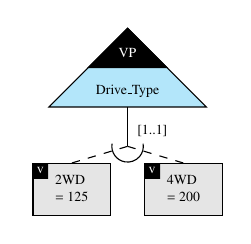
\begin{tikzpicture}
   \nodeVP{drivetype}{at={(0,0)}}{Drive\_Type};
   \nodeV{2wd}{below left=0.3cm of via_drivetype}{2WD}{= 125};
   \draw [dashed](via_drivetype)--(2wd.north);
   \nodeV{4wd}{below right=0.3cm of via_drivetype}{4WD}{= 200};
   \draw [dashed](via_drivetype)--(4wd.north);
  \end{tikzpicture}
 \end{center}

\vfill
\begin{exampleblock}{}
\begin{lstlisting}
  (1) { vp(VP,G) } :- vp_def(VP), group(G). 
  (2) 1 { v(V,G) : v_def(V,VP,_) } 1 :- vp(VP,G).
\end{lstlisting}
\end{exampleblock}
\vfill
\begin{itemize}
\item (1)
  各車種\code{G},各装備タイプ\code{VP}に対して,
  \code{G}が\code{VP}を装備することを意味するアトム
  \code{vp(VP,G)}を導入.
\item (2)
  各車種\code{G},各装備タイプ\code{VP}に対して,
  \code{vp(VP,G)}が成り立つならば,
  \code{G}が\code{VP}のオプション\code{V}を装備することを意味する
  アトム\code{v(V,G)}を導入し,そのうちの
  ちょうど1個を装備することを強制する.
\end{itemize}
\end{frame}
%%%%%%%%%%%%%%%%%%%%%%%%%%%%%%%%%%%%%%%%%%%%%%%%%%%%
% \begin{frame}[fragile]{制約のASP符号化}
% \begin{exampleblock}{範囲制約}\small
% \begin{lstlisting}
%  1 { v(V,G) : v_def(V,VP,_) } 1 :- vp(VP,G).
% \end{lstlisting}
% \end{exampleblock}
% \begin{itemize}
%  \item アトム\code{vp(VP,G)}は,各車種\code{G},各装備タイプ\code{VP}に対して,
%        \code{G}が\code{VP}を装備することを意味する.
%  \item 

% \end{itemize}
% % \begin{exampleblock}{依存制約}\small
% % \begin{lstlisting}
% %  1 { v(V,G) : v_def(V,VP,_) } 1 :- vp(VP,G).
% % \end{lstlisting}
% % \end{exampleblock}
% \begin{exampleblock}{燃費制約}\small
% \begin{lstlisting}
%  iwr(S,G) :- S = #sum { IWR,V : v(V,G), v_def(V,_,IWR) },
%              LB <= S, S <= UB, lb_iwr(LB), ub_iwr(UB), group(G).
%  :- not 0 #sum { (FE-t)*SV,FE,SV,G : fe(FE,G), sv(SV,G) }.
% \end{lstlisting}
% \end{exampleblock}
% \begin{itemize}
%  \item 
% \end{itemize}
% \end{frame}
%%%%%%%%%%%%%%%%%%%%%%%%%%%%%%%%%%%%%%%%%%%%%%%%%%%%
\begin{frame}[fragile]{目的関数のASP符号化}
\begin{exampleblock}{}\small
\begin{lstlisting}
 (3) #preference (max_sv, more(weight)) { SV,G :: sv(SV,G) }.
 (4) #preference (min_op, less(weight)) { 1,V :: used_v(V) }.
 (5) #preference (all, pareto) { **max_sv; **min_op}.
 (6) #optimize(all). 
\end{lstlisting}
\end{exampleblock}
\begin{itemize}
 \item (3) 予想販売台数の最大化を\code{max\_sv}という名称で定義している.\\
       アトム\code{sv(SV,G)}は,車種\code{G}の予想販売台数が\code{SV}であることを意味する. 
 \item (4) 装備オプションの最小化を\code{min_op}という名称で定義している.\\
       アトム\code{used\_v(V)}は,装備オプション\code{V}がいずれかの車種において
       実装されたことを意味する.
 \item (5) \code{max\_sv}と\code{min\_op}の2目的のパレート最適化を\code{all}という
       名称で定義している.
 \item (6) 選好名称\code{all}について最適化することで,多目的CAFE問題のパレート最適解を得る.
\end{itemize}
\end{frame}
%%%%%%%%%%%%%%%%%%%%%%%%%%%%%%%%%%%%%%%%%%%%%%%%%%%%
\begin{frame}{実験概要}
 \begin{itemize}
  \item 考案したASP符号化の有効性を評価するために,実行実験を行った.
% 問題の規模がわかるように	
 \end{itemize}

\begin{itemize}
\item ベンチマーク問題(計15問)
  \begin{itemize}
  \item 企業から提供された問題(3問)に対して
  \item 5通りのCAFE基準値$t\in\{8.5, 9.0, 9.5, 10.0, 10.5km/L\}$を適用
  \item 車種の数$n = 3$
  \end{itemize}
  \begin{exampleblock}\small
    \centering
    \begin{tabular}{ ll|r r r }
      問題名 & サイズ &  \#装備タイプ & \#装備オプション& \#依存制約\\ \hline
      small	 & 小規模   &   8 &   21  &   4	\\
      medium & 実用規模 &  86 &  226  & 147	\\
      big    & 大規模   & 315 & 1,337 &   0
    \end{tabular}
  \end{exampleblock}
 \item ASPシステム
       \begin{itemize}
	\item \textit{clingo-5.4.0} + \textit{asprin-3.1.1}
       \end{itemize}
 \item 制限時間
       \begin{itemize}
	\item 1問あたり3時間
       \end{itemize}
 \item 実験環境: Mac mini (3.2GHz, Intel Core i7, 64GB メモリ)
\end{itemize}
\end{frame}
%%%%%%%%%%%%%%%%%%%%%%%%%%%%%%%%%%%%%%%%%%%%%%%%%%%%
\begin{frame}{小規模な問題での実験結果}
 \begin{exampleblock}{}
  \centering
  % \renewcommand{\arraystretch}{0.9}
  % \tabcolsep = 0.9mm
  \begin{tabular}{c|r|rr}
   問題   & CAFE値  & パレート最適解 & CPU時間(秒) \\
          & (km/L)  & の総数  &  \\ \hline
   small  & 8.5   & 8             & 35.136     \\
   small  & 9.0   & 5             & 1085.354   \\
   small  & 9.5   & --            & Timeout    \\
   small  & 10.0  & 1             & 1.863      \\
   small  & 10.5  & 0             & 0.221      \\ 
  \end{tabular}
 \end{exampleblock}
 \begin{itemize}
  \item 5問中4問でパレート最適解を全列挙することに成功した.
  \item medium 以上の問題ではパレート解は得られたが,最適解は得られなかった.
 \end{itemize}
\end{frame}
%%%%%%%%%%%%%%%%%%%%%%%%%%%%%%%%%%%%%%%%%%%%%%%%%%%%
\begin{frame}{まとめ}
 ASP に基づく多目的 CAFE 問題ソルバーの実装と評価について述べた.   
 \begin{block}{研究内容}
 \begin{itemize}
  \item ASP 言語の表現力の高さを活かし,多目的 CAFE 問題の制約と
	目的関数を簡潔に表現できることを確認した.
  \item 企業から提供を受けたベンチマーク問題を用いて評価実験を行った結果,
	小規模な問題に対して,パレート 最適解を全列挙をすることができた.
 \end{itemize}
 \end{block}

 \begin{exampleblock}{今後の課題}
  \begin{itemize}
   \item ソルバーの高速化および大規模な問題への対応
   \item ZEVクレジット制約の追加や,Minimal perturbation問題への拡張
  \end{itemize}
 \end{exampleblock}
\end{frame}
%%%%%%%%%%%%%%%%%%%%%%%%%%%%%%%%%%%%%%%%%%%%%%%%%%%% 
\appendix
\backupbegin
%%%%%%%%%%%%%%%%%%%%%%%%%%%%%%%%%%%%%%%%%%%%%%%%%%%%
\begin{frame}{}
  \vskip 3em
  \begin{center}\LARGE
    ご清聴ありがとうございました.    
  \end{center}
\end{frame}
%%%%%%%%%%%%%%%%%%%%%%%%%%%%%%%%%%%%%%%%%%%%%%%%%%%%
\begin{frame}{ASPの構文}
  \begin{alertblock}{}\centering
    ASPの言語は論理プログラムをベースとしている~\footnotemark.
  \end{alertblock}
  \begin{itemize}
  \item \structure{\bf 論理プログラム}とは,以下の\structure{\bf ルール}の有限集合である.
    \begin{center}
      \begin{minipage}[c]{0.7\textwidth}
        \begin{block}{}\centering
          $a_0$\quad\code{:-} \quad$a_1$\code{,}\ldots\code{,}$a_m$\code{,}
          \ \code{not}~$a_{m+1}$\code{,}\ldots\code{,} \code{not}~$a_n$\code{.}
        \end{block}        
      \end{minipage}
   \end{center}\vfill
    $0 \leq m \leq n$ であり,各 $a_i$ はアトム,
    \code{not}は\structure{\bf デフォルトの否定},\\
    ``\code{,}''は連言(AND)を表す.
  \item \alert{\bf 直感的な意味}は,
    「$a_1,\ldots,a_m$がすべて成り立ち,
    $a_{m+1},\ldots,a_n$のそれぞれが成り立たないならば,
    $a_0$が成り立つ」である.
  \item ボディが空のルールを\structure{\bf ファクト}と呼び,``\code{:-}''は省略できる.
  \item ヘッドが空のルールを\structure{\bf 一貫性制約}と呼ぶ.例えば,
    ``\code{:-} $a_1$\code{,} \code{not}~$a_{2}$''は,
    「$a_1$が成り立つならば,$a_2$が成り立つ」を意味する.
  \end{itemize}
  \footnotetext{本発表では標準論理プログラムを単に論理プログラムと呼ぶ.}
\end{frame}
%%%%%%%%%%%%%%%%%%%%%%%%%%%%%%%%%%%%%%%%%%%%%%%%%%%%
\begin{frame}{ASPの拡張構文}
  \begin{alertblock}{}\centering
    組合せ最適化問題を解くための便利な構文が用意されている.
  \end{alertblock}

  \begin{itemize}
 \item \structure{\bf 選択子}
   \begin{center}
     \code{\{}$a_1$\code{;}\ldots\code{;}$a_n$\code{\}}
   \end{center}
   アトム集合 $\{a_1,\dots,a_n\}$
   の任意の部分集合が成り立つことを意味する.
 \item \structure{\bf 個数制約}
   \begin{center}
     $lb$\ \code{\{}$a_1$\code{;}\ldots\code{;}$a_n$\code{\}}\ $ub$
   \end{center}
   $a_1,\dots,a_n$ のうち,
   $lb$個以上,$ub$個以下が成り立つことを意味する.
 % \item \structure{\bf 重み付き個数制約}
 %   \begin{center}
 %     $t$ \code{= \#sum} \code{\{} $w_1$\code{:}$a_1$\code{;}\ldots\code{;}$w_n$\code{:}$a_n$ \code{\}}
 %   \end{center}
 %   $a_1,\dots,a_n$のうち,
 %   成り立つアトムの重み和が項$t$に等しくなることを意味する.
 \item \structure{\bf \code{\#preference}文}
       \begin{center}
	\code{\#preference(}$s,t$\code{)\{}$e_1,\dots,e_n$\code{\}.}
       \end{center}
       $s$ は選好名称,$t$ は選好タイプ,$e_j$ は要素を表す.\\
       選好タイプには\code{subset}, \code{less(weight)}, \code{more(weight)}, 
       \code{pareto}などがあらかじめ用意されている.
       % \code{\#optimize(}$s$\code{)}と記述することによって,
       % 選好名称$s$ について最適な解集合を得ることができる.
 \end{itemize}
\end{frame}
%%%%%%%%%%%%%%%%%%%%%%%%%%%%%%%%%%%%%%%%%%%%%%%%%%%%
\begin{frame}[fragile]{制約のASP符号化: 依存制約(要求・排他)}
 \begin{center} 
 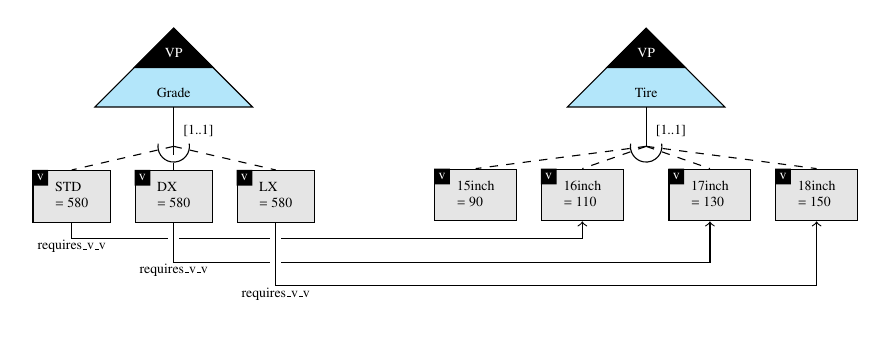
\begin{tikzpicture}
 % Grade
  \nodeVP{grade}{at={(0,0)}}{Grade};
  \nodeV{dx}{below=0.3cm of via_grade}{DX}{= 580};
  \draw[dashed](via_grade)--(dx.north);
  \nodeV{std}{left=0.3cm of dx}{STD}{= 580};
  \draw[dashed](via_grade)--(std.north);
  \nodeV{lx}{right=0.3cm of dx}{LX}{= 580};
  \draw[dashed](via_grade)--(lx.north);

  % Tire
  \nodeVP{tire}{right=6cm of grade}{Tire};
  \nodeV{16inch}{below left=0.4cm of via_tire}{16inch}{= 110};
  \nodeV{17inch}{below right=0.4cm of via_tire}{17inch}{= 130};
  \nodeV{15inch}{left=0.3cm of 16inch}{15inch}{= 90};
  \nodeV{18inch}{right=0.3cm of 17inch}{18inch}{= 150};
  \draw [dashed](via_tire)--(15inch.north);
  \draw [dashed](via_tire)--(16inch.north);
  \draw [dashed](via_tire)--(17inch.north);
  \draw [dashed](via_tire)--(18inch.north);

  % require
  \draw[->] (std.south)--++(0,-0.2) node[below=-1mm] {\tiny{requires\_v\_v}} -|(16inch.south);
  \draw[white,line width=4pt](dx.south) ++(0,-0.1)--++(0,-0.5);
  \draw[->] (dx.south)--++(0,-0.5) node[below=-1mm] {\tiny{requires\_v\_v}} -|(17inch.south);
  \draw[white,line width=4pt] (lx.south) ++(0,-0.1)--++(0,-0.8);
  \draw[->] (lx.south)--++(0,-0.8) node[below=-1mm] {\tiny{requires\_v\_v}} -|(18inch.south);
 \end{tikzpicture}
 \end{center}

\vfill
\begin{exampleblock}{}
\begin{lstlisting}
  (a) :- require_v_v(V1,V2), v(V1,G), not v(V2,G).
  (b) :- exclude_v_v(V1,V2), v(V1,G), v(V2,G).
\end{lstlisting}
\end{exampleblock}
\vfill
\begin{itemize}
\item (a)
  要求関係\code{require_v_v(V1,V2)}が与えられたとき,
  車種\code{G}がオプション\code{V1}を実装するならば,
  \code{G}は\code{V2}も実装しなければならない.
\item (b)
  排他関係\code{exclude_v_v(V1,V2)}が与えられたとき,
  車種\code{G}が\code{V1}と\code{V2}を
  同時に実装することはない.
\end{itemize}
\end{frame}
%%%%%%%%%%%%%%%%%%%%%%%%%%%%%%%%%%%%%%%%%%%%%%%%%%%%
\begin{frame}[fragile]{制約のASP符号化: 燃費制約}
\begin{exampleblock}{}\small
\begin{lstlisting}
  (c) iwr(S,G) :- 
         S = #sum { IWR,V : v(V,G), v_def(V,_,IWR) }, group(G).
  (d) fe(FE,G) :- iwr(S,G), fe_map(S,FE).
  (e) sv(SV,G) :- iwr(S,G), sv_map(S,SV).
  (f) :- not 0 #sum { (FE-t)*SV,FE,SV,G : fe(FE,G), sv(SV,G) }.
\end{lstlisting}
\end{exampleblock}
\vfill
\begin{itemize}
\item (c)
  アトム\code{iwr(S,G)}は,車種\code{G}に実装されるオプションのIWR値の
  総和が\code{S}であることを表す.
\item (d, e)
  \code{fe(FE,G)}と\code{sv(SV,G)}は,
  それぞれ車種\code{G}の燃費が\code{FE},予想販売台数が\code{SV}
  であることを表す.
\item (f)
  CAFE方式の制約式を以下のように変形し,
  ASPの重み付き個数制約で表現している.ただし,$t$はCAFE基準値
  \[\sum_{i=1}^{n} (FE_{i}-t)\cdot SV_{i} \geq 0\]
\end{itemize}
\end{frame}
%%%%%%%%%%%%%%%%%%%%%%%%%%%%%%%%%%%%%%%%%%%%%%%%%%%%
\begin{frame}{単目的CAFE問題における実験結果: 予想販売台数}
\begin{itemize}%\small
 \item 目的関数は,予想販売台数の最大化のみ
\end{itemize}	
\begin{exampleblock}{}
  \centering
  \scriptsize
  \renewcommand{\arraystretch}{1.1}
  \tabcolsep = 7mm
  \begin{tabular}{l|r|r}
  \lw{問題名} & CAFE  & 予想販売台数 \\ 
              & 基準値 &   \\\hline    
   small & 8.5   & 6,021*       \\
   small & 9.0   & 5,007*       \\
   small & 9.5   & 2,688*       \\
   small & 10.0  & 1,318*       \\
   small & 10.5  & UNSAT    \\\hline
   medium & 8.5  & 6,021        \\
   medium & 9.0  & 5,595        \\
   medium & 9.5  & 3,430        \\
   medium & 10.0 & 2,250        \\
   medium & 10.5 & 1,845        \\\hline
   big & 8.5     & 3,877        \\
   big & 9.0     & 4,623        \\
   big & 9.5     & 3,121        \\
   big & 10.0    & 2,064        \\
   big & 10.5    & 904        
  \end{tabular}
\end{exampleblock}
\vfill
\end{frame}
%%%%%%%%%%%%%%%%%%%%%%%%%%%%%%%%%%%%%%%%%%%%%%%%%%%%
% \begin{frame}[fragile]{制約のASP符号化: 燃費制約}
% \begin{exampleblock}{}\small
% \begin{lstlisting}
% ub_vp(UB,VP) :- UB = #max { IWR,V : v_def(V,VP,IWR) }, vp_def(VP).
% ub_iwr(S) :- S = #sum { UB,VP : ub_vp(UB,VP) }.
% iwr(S,G) :- S = #sum { IWR,V : v(V,G), v_def(V,_,IWR) },
%             LB <= S, S <= UB, lb_iwr(LB), ub_iwr(UB), group(G).
% fe(FE,G) :- iwr(S,G), fe_map(S,FE).
% sv(SV,G) :- iwr(S,G), sv_map(S,SV).
% :- not 0 #sum { (FE-t)*SV,FE,SV,G : fe(FE,G), sv(SV,G) }.
% \end{lstlisting}
% % lb_vp(LB,VP) :- LB = #min { IWR,V : v_def(V,VP,IWR) }, vp_def(VP).
% % lb_iwr(S) :- S = #sum { LB,VP : lb_vp(LB,VP), require_vp(VP) }.
% \end{exampleblock}
% \vfill
% \begin{itemize}
%  \item アトム\code{iwr(S,G)}は,車種\code{G}に実装されるオプションのIWR値の
%        総和が\code{S}であることを表す.
%  \item \code{fe(FE,G)}と\code{sv(SV,G)}は,
%        それぞれ車種\code{G}の燃費が\code{FE},予想販売台数が\code{SV}
%        であることを表す.
%  \item CAFE方式の制約式を以下のように変形し,
%        ASPの重み付き個数制約で表現している.ただし,$t$はCAFE基準値
%        \[\sum_{i=1}^{n} (FE_{i}-t)\cdot SV_{i} \geq 0\]
% \end{itemize}
% \end{frame}
%%%%%%%%%%%%%%%%%%%%%%%%%%%%%%%%%%%%%%%%%%%%%%%%%%%%
% \begin{frame}{基礎化後のルール数}
%  \begin{exampleblock}{}\centering 
%   \renewcommand{\arraystretch}{1.2}
%   \tabcolsep = 4mm
%   \begin{tabular}{crr} 
%    問題名    & 基本符号化       & 改良符号化    \\ \hline
%    small    &  83,520 (1.00)  & 32,855 (0.39) \\ 
%    medium   &  93,017 (1.00)  & 56,940 (0.61) \\
%    big	    & 155,654 (1.00)  & 42,190 (0.27) \\ 
%   \end{tabular}
%  \end{exampleblock}
%  \begin{itemize}
%   \item 改良符号化は,基本符号化と比較して,基礎化後のルール数を
% 	少なく抑えられている.
%   \item 特にbigでは,70\%以上のルール数の削減に成功している.
%  \end{itemize}
%  % \begin{alertblock}{}
%  %  このルール数の削減が,改良符号化の大規模問題に対する優位性につながっていると考えられる.
%  % \end{alertblock}
% \end{frame}
%%%%%%%%%%%%%%%%%%%%%%%%%%%%%%%%%%%%%%%%%%%%%%%%%%%%
\backupend
\end{document}

%%% Local Variables:
%%% mode: japanese-latex
%%% TeX-master: t
%%% End:
